\section{Results}

\textbf{In this section we will apply the model described in the previous section to a times series from 1997-2020. It includes major indices all representing distinct asset classes. Since calculations for this section is still underway it is omitted from this version.}


\subsection{Data}

Sktiser index data på log scala + evt. tabel over aktivers perfomance over periode - thats it.

\begin{figure}[H]
    \centering
    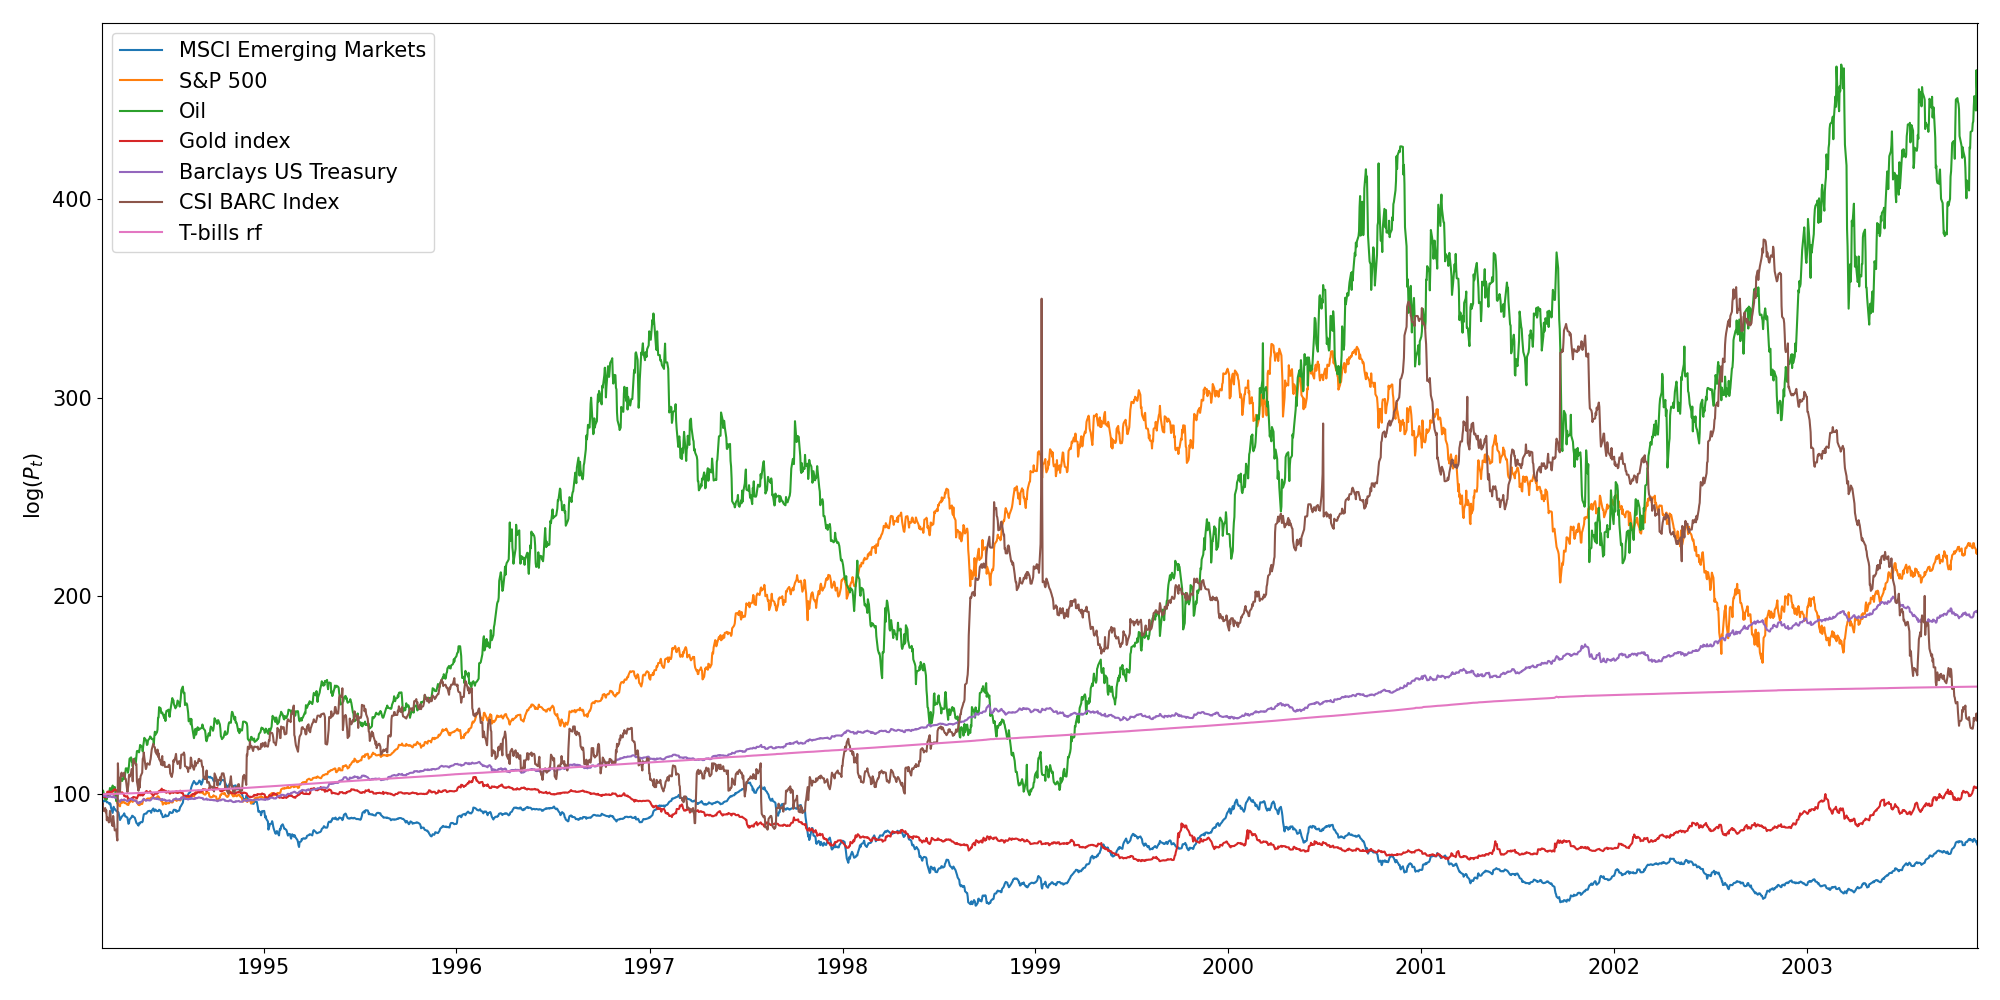
\includegraphics[width=1\textwidth]{analysis/portfolio_exercise/images/asset_vals_insample.png}
    \caption[Log of historical asset prices during the in-sample period]{Log of historical asset prices during the in-sample period.}
    \label{fig:MPC_data}
\end{figure}


\begin{figure}[H]
    \centering
    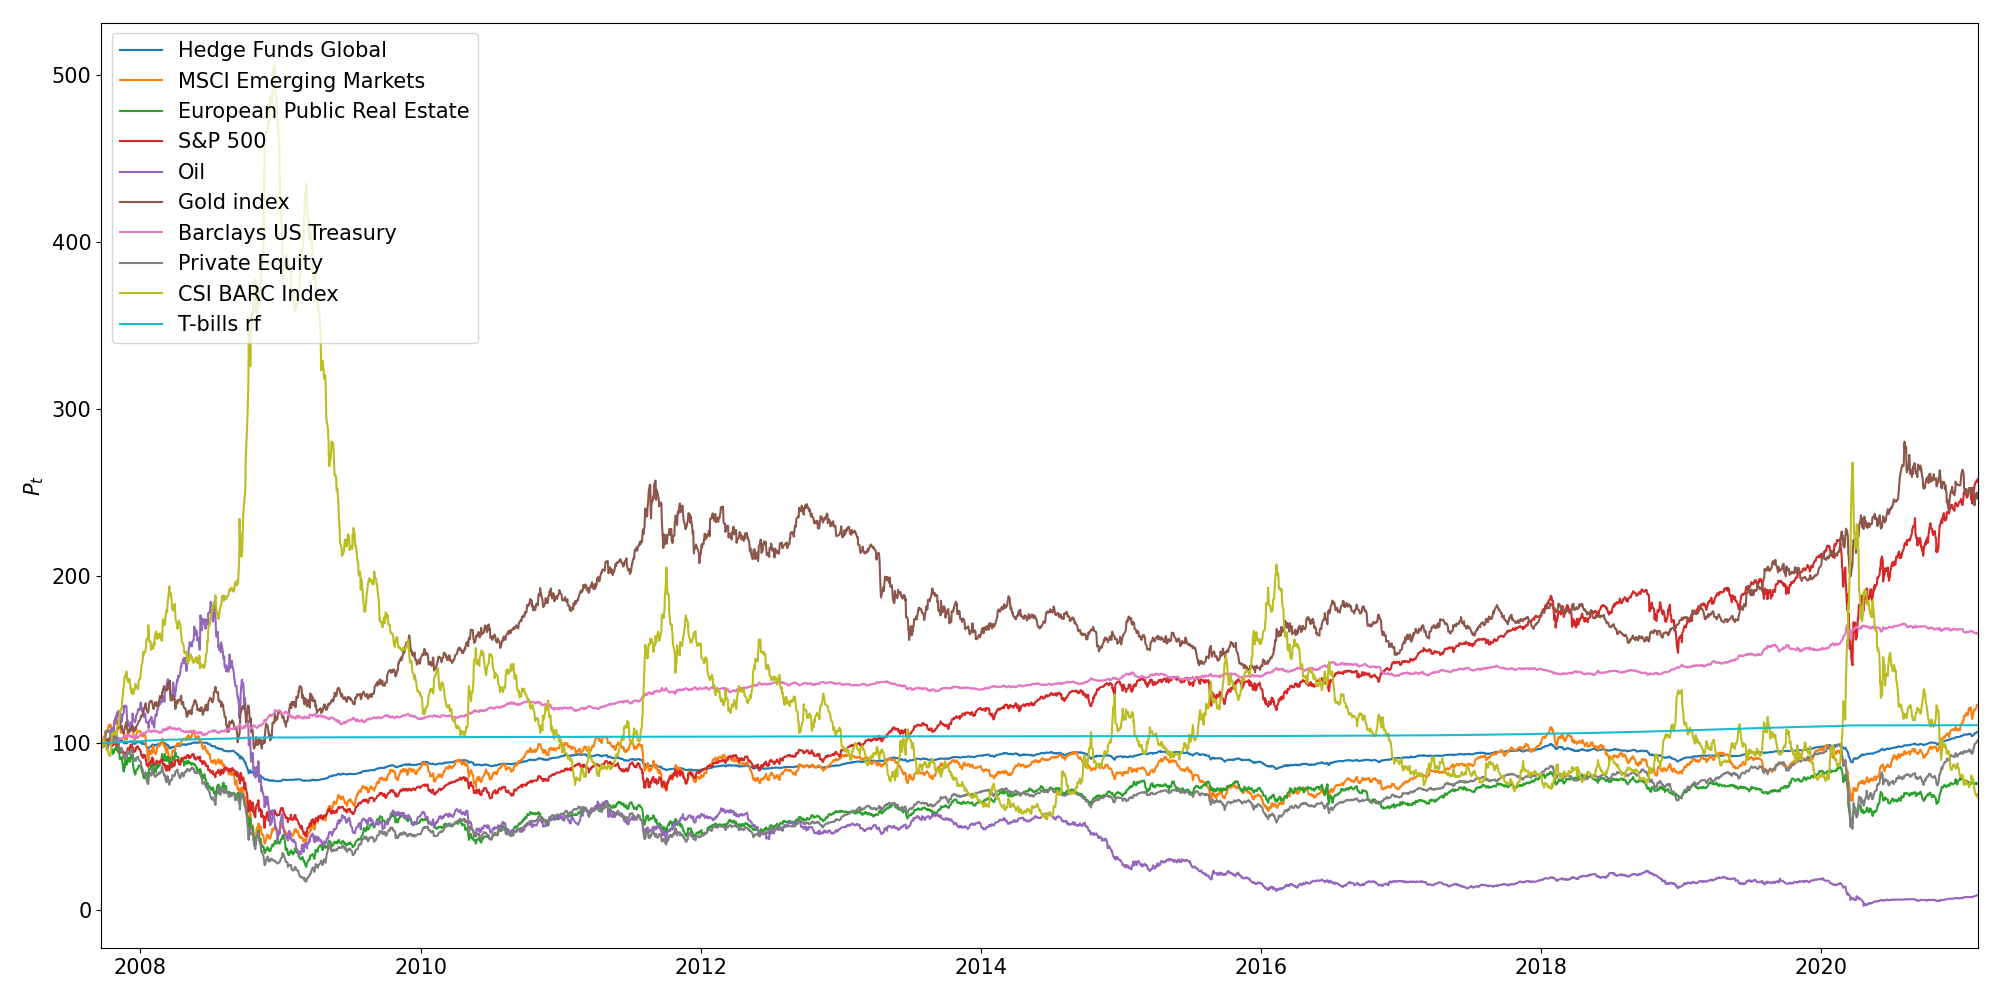
\includegraphics[width=1\textwidth]{analysis/portfolio_exercise/images/asset_vals_oos.png}
    \caption[Log of historical asset prices during the out-of-sample period]{Log of historical asset prices during the out-of-sample period.}
    \label{fig:MPC_data}
\end{figure}

In \cref{tab:MPC_asset_performance} we show annualized\footnote
{Daily returns are analyzed using
\begin{flalign*}
    \mu_{annual} &= (1+\mu_{daily})^{1/252}-1 \\
    \Sigma_{annual} &= {\Sigma}_{daily} * 252
\end{flalign*}
}
asset performance.

\begin{table}[H]
\centering
\caption[Annualized
performance for each asset during the out-of-sample period]{Annualized
performance for each asset during the out-of-sample period. All measures are in excess of the risk-free rate.}
\begin{tabular}{lrrrrrrr}
\toprule
{} &  return &     std &  excess\_return &  excess\_std &  sharpe &  max\_drawdown &  calmar\_ratio \\
\midrule
MSCI World            &  0.0338 &  0.1638 &         0.0180 &      0.1641 &  0.1094 &        0.5907 &        0.0304 \\
MSCI Emerging Markets &  0.0591 &  0.1869 &         0.0429 &      0.1872 &  0.2291 &        0.6606 &        0.0649 \\
S\&P 500               &  0.0459 &  0.1923 &         0.0299 &      0.1925 &  0.1553 &        0.5678 &        0.0527 \\
Oil                   & -0.0800 &  0.3928 &        -0.0941 &      0.3929 & -0.2395 &        0.9852 &       -0.0955 \\
Gold index            &  0.0929 &  0.1681 &         0.0762 &      0.1680 &  0.4537 &        0.4462 &        0.1708 \\
Barclays US Treasury  &  0.0427 &  0.0443 &         0.0268 &      0.0440 &  0.6099 &        0.0717 &        0.3742 \\
CSI BARC Index        & -0.0428 &  0.3155 &        -0.0573 &      0.3153 & -0.1818 &        0.8925 &       -0.0642 \\
port\_val              &  0.0530 &  0.0967 &         0.0370 &      0.0965 &  0.3828 &        0.2671 &        0.1384 \\
\bottomrule
\end{tabular}

\label{tab:MPC_asset_performance}
\end{table}


\subsection{In-sample training: Tuning hyperparameters}



\begin{itemize}
    \item Sample period
    \item method - what do we maximize
    \item go over each tuning parameter separately.
\end{itemize}

\textbf{Maximize portfolio Sharpe, excess return and minimize annual turnover over the hyperparameters}

\subsection{Out-of-sample results}

\begin{itemize}
    \item Plot allocations
    \item Plot portfolio performance
    \item Table summarizing KPIs
\end{itemize}

\begin{figure}[H]
    \centering
    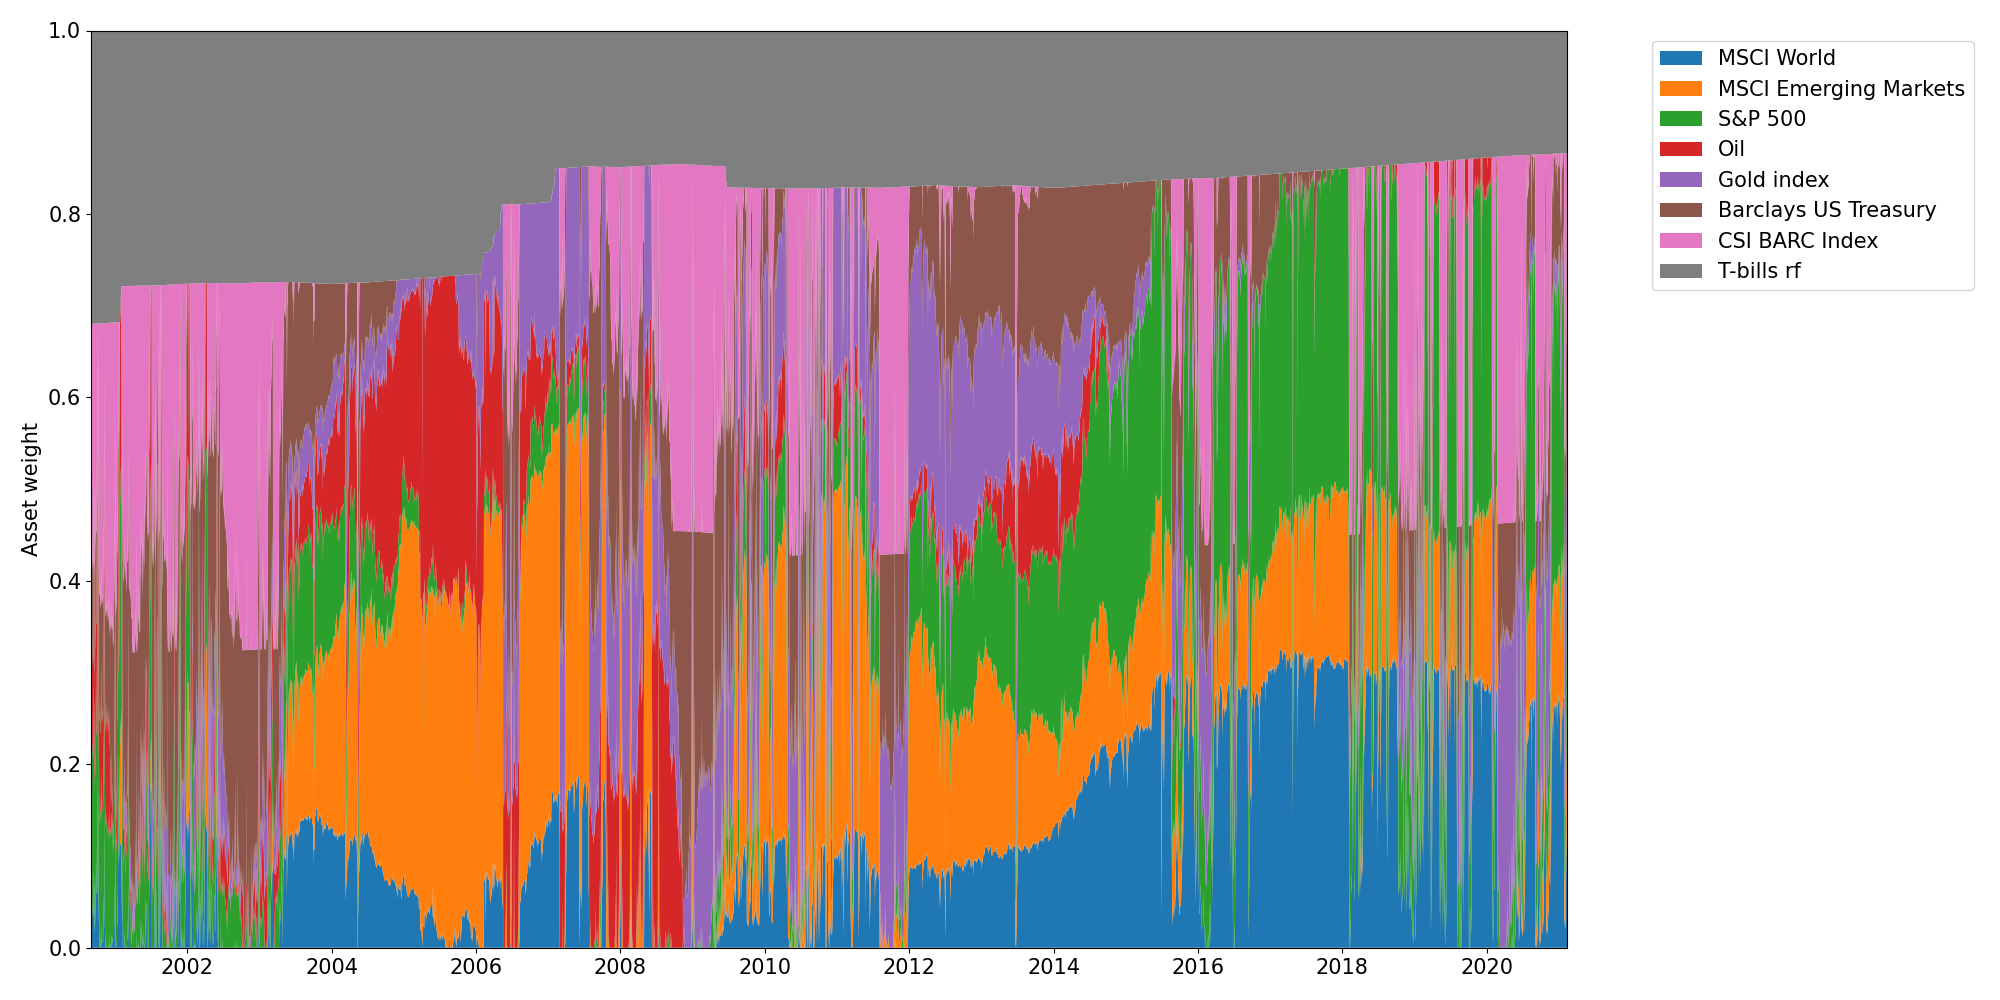
\includegraphics[width=1\textwidth]{analysis/portfolio_exercise/images/port_weights.png}
    \caption[Asset weights over time for a long-only portfolio]{Asset weights over time for a long-only portfolio.}
    \label{fig:MPC_port_weights}
\end{figure}


\subsubsection{Comparison}



\subsubsection{Notes to self}


\textbf{Consider using rolling estimation of state sequence where only 1 new state is detected each time step(like in BP) - current approach estimates a new state sequence over entire rolling window at each timestep, which might make estimated means and covariances more unstable. Also, do we include rf in theestimates of mu and covariance matrix or how do we handle that asset?}

\textbf{Consider adding estimation section for portfolio allocation as in BP - trained on the same in-sample data as the rest.}